\documentclass[a4paper]{article}

\usepackage{tikz}
\usetikzlibrary{arrows}
\usetikzlibrary{trees}


\usepackage{textcomp}
\usepackage{graphicx}
\graphicspath{ {/media/sf_Ubuntu_Shared/}{/home/brandon/Documents/texFiles/examples/} }

\newcommand{\numpy}{{\tt numpy}}	% tt font for numpy

\topmargin -.5in
\textheight 9in
\oddsidemargin -.25in
\evensidemargin -.25in
\textwidth 7in

\begin{document}
	\author{Brandon Thompson 5517}
	\title{Assignment 2: Due 9/17/19}
	\maketitle

	\medskip

	Find a suitable \textit{state representation, a set of operations} and draw a
	\textit{search tree} for the folloing problem:\\

	Consider the purchare of a soft drink from a maxhine. As you put coins into the machine,
	it makes a transition from one state to another.\\
	Let's assume that only quarters and nickles are acceptable to the machine and 55 cents
	are required for a drink.

	\begin{itemize}
		\item Set of operators.
		\begin{enumerate}
			\item Add nickel (5 \textcent).
			\item Add quarter (25 \textcent).
		\end{enumerate}
		\item States
		\begin{enumerate}
			\item Start state $(0)$.
			\item Goal state  $(55)$.
		\end{enumerate}
	\end{itemize}

	\begin{figure}[ht]
		\centering
		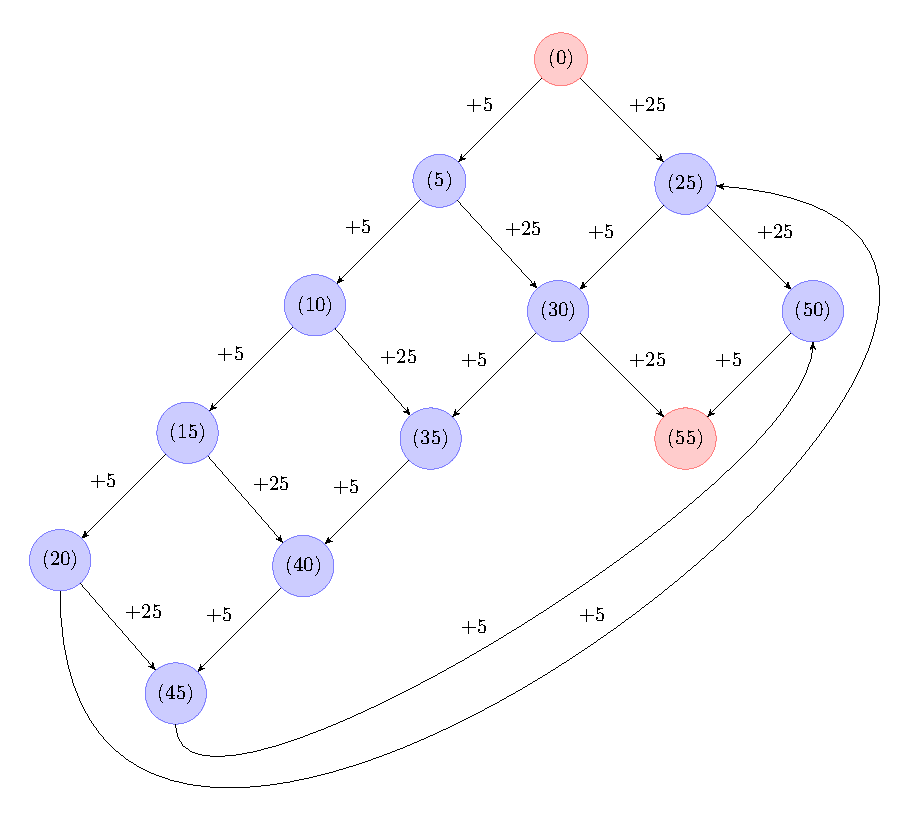
\includegraphics[width=0.6\textwidth]{tikz_state_machine}
		\caption{State space representation of drink machine, start and end nodes are red}
		\label{fig:tikz_state_machine}
	\end{figure}
	
	\begin{figure}[ht]
		\centering
		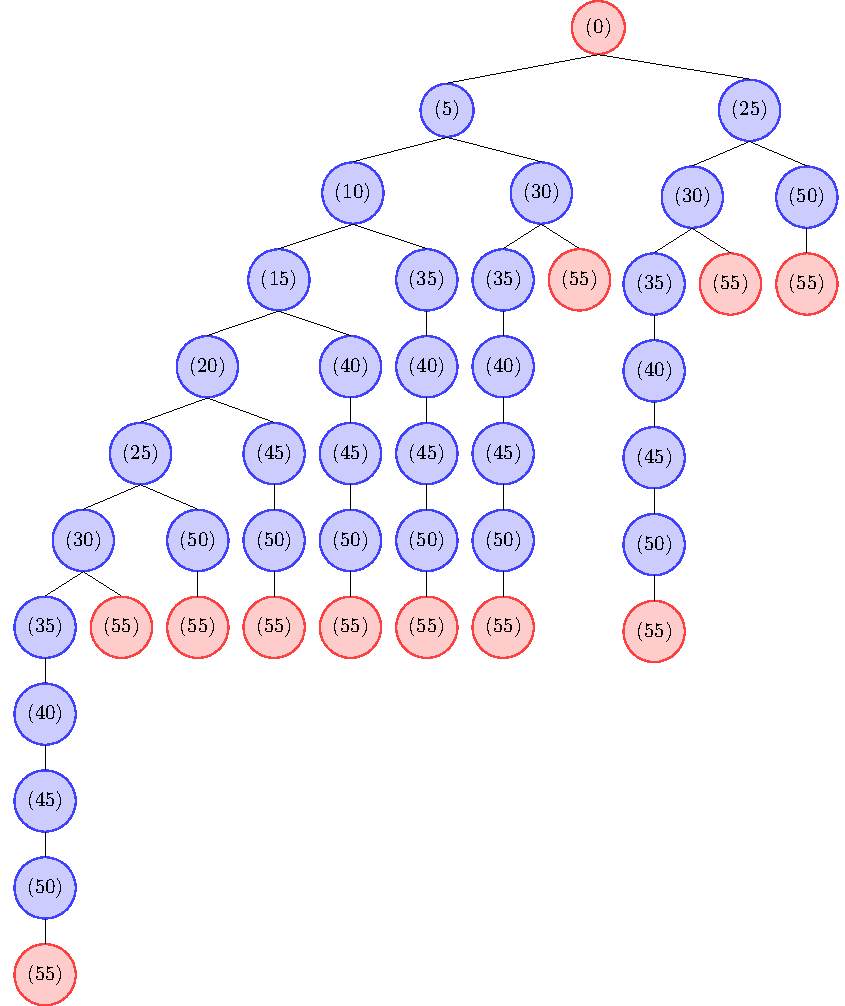
\includegraphics[width=0.6\textwidth]{tikz_search_tree}
		\caption{Search tree of drink machine, start and end nodes are red}
		\label{fig:tikz_search_tree}
	\end{figure}

	

\end{document}
